\documentclass[a4paper, 10pt, dvipdfmx]{jlreq}

\usepackage{amsmath,amsfonts,amssymb}
\usepackage{bm}
\usepackage{mathtools}
\usepackage{siunitx}
\usepackage[dvipdfmx]{graphicx}
\usepackage[dvipdfmx]{color}
\usepackage[dvipdfmx, colorlinks=true, allcolors=blue]{hyperref}
\usepackage{listings, jlisting}
\usepackage{tikz}
\usepackage{physics}
\usepackage{url}

\Urlmuskip=0mu plus 10mu
\allowdisplaybreaks[4]
\frenchspacing
\definecolor{OliveGreen}{rgb}{0.0,0.6,0.0}
\definecolor{Orenge}{rgb}{0.89,0.55,0}
\definecolor{SkyBlue}{rgb}{0.28, 0.28, 0.95}
\lstset{
  language={c++},
  basicstyle={\ttfamily},
  identifierstyle={\small},
  ndkeywordstyle={\small},
  frame=single,
  breaklines=true,
  numbers=left,
  xrightmargin=0zw,
  xleftmargin=3zw,
  numberstyle={\scriptsize},
  lineskip=-0.9ex,
  keywordstyle={\small\bfseries\color{SkyBlue}},  
  commentstyle={\color{OliveGreen}}, 
  stringstyle={\small\ttfamily\color{Orenge}}    
}

\begin{document}

\title{2012年度 大問3}
\author{hari64boli64 (hari64boli64@gmail.com)}
\date{\today}
\maketitle

\section{問題}

ポアソン過程 計算問題

(注意力が無い人間には捨て問だと思う。私は注意力が無さ過ぎて三日掛かった)

\section{解答}

\subsection*{(1)}

\begin{align*}
  a(P(t,n-1)-P(t,n))+b((n+1)P(t,n+1)-nP(t,n))
\end{align*}

\subsection*{(2)}

\begin{align*}
  M(t)=\frac{a}{b}+\qty(\lambda-\frac{a}{b})e^{-bt}
\end{align*}

\subsection*{(3)}

\begin{align*}
  \pdv{G(t,s)}{s}=(s-1)\qty(aG(t,s)-b\pdv{G(t,s)}{s})
\end{align*}

$\bar{G}(s)=1$より、

\begin{align*}
  \bar{G}(s)=e^{\frac{a}{b}(s-1)}
\end{align*}

\subsection*{(4)}

$G(0,s)=e^{\lambda (s-1)}$より、

\begin{align*}
  K(s-1) & =e^{\qty(\lambda-\frac{a}{b})(s-1)} \\
  K(x)   & =e^{\qty(\lambda-\frac{a}{b})x}
\end{align*}

\begin{align*}
  P(t,n) & =\frac{1}{n!}\pdv{^n}{s^n}G(t,s)\eval_{s=0} \\
         & =\frac{1}{n!}M(t)^n e^{-M(t)}
\end{align*}

図\ref{img:simulation}は、シミュレーション値と理論値が一致しすぎて、青と赤が重なり紫になっている。

\begin{figure}[htbp]
  \begin{center}
    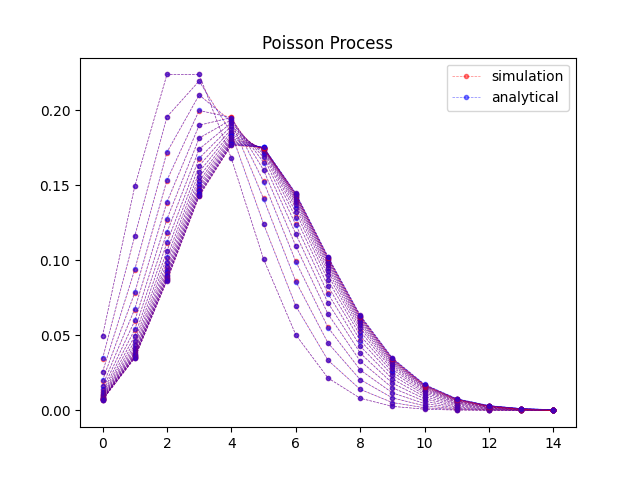
\includegraphics[height=80mm]{3.png}
    \caption{simulation}
    \label{img:simulation}
  \end{center}
\end{figure}

\section{知識}

なし

\section{おまけ}

\lstinputlisting[caption=simulation,label=code:simulation,language=Python]{3.py}

\end{document}
